\chapter{Testy sposobów komunikacji radiowej}
\label{cha:teoria}

\section{Bluetooth}
%http://bluetoothinsight.blogspot.com/2008/01/bluetooth-power-classes.html
\section{Eksperymenty}
\subsection{Wykorzystane urządzenia}
\begin{enumerate}
	\item Smartphone Sony Xperia Z1 Compact (D5503) - odbiornik\\				
	Dane techniczne:
	\begin{itemize}
		\item Częstotliwość - 2,4GHz
		\item Przyrost siły sygnału z anteny - 2dBi
	\end{itemize}
	\item Router TP-Link TD-W8970 - nadajnik\\
	Dane techniczne:
	\begin{itemize}
		\item Częstotliwość - 2,4GHz
		\item Dwie zewnętrzne anteny kierunkowe
		\item Przyrost siły sygnału z anteny - 4dBi
		\item Siła transmitera - 16.5dBm					
	\end{itemize}
	\item Router TP-Link TL-WA701ND - nadajnik\\
	Dane techniczne:
	\begin{itemize}
		\item Częstotliwość - 2,4GHz
		\item Jedna zewnętrzna antena kierunkowa
		\item Przyrost siły sygnału z anteny - 2dBi
		\item Siła transmitera - 15dBm					
	\end{itemize}
	\item Smartphone Grand 2 (G7102) - nadajnik\\
	Dane techniczne:
	\begin{itemize}
		\item Częstotliwość - 2,4GHz
		\item Jedna antena wbudowana
		\item Przyrost siły sygnału z anteny - 0dBi
		\item Siła transmitera - 10dBm					
	\end{itemize}
\end{enumerate}
\subsection{Warunki}
Wszystkie pomiary wykonywane były w pomieszczeniu zamknięty, bez przeszkód na drodze sygnału, dlatego jako margines zaniku sygnału została przyjęte wartość 22 dBm. Inne straty (np interferencja sygnałów z routerów) zostały pominięte i ich wykrycie jest jednym z celów eksperymentu.
\subsection{Cele}
Celem eksperymentu jest ustalenie, jak zmierzona i obliczona, przy użyciu siły sygnałów, odległość między odbiornikiem i transmiterami odnosi się do odległości rzeczywistej. Dodatkowo, będę się starał ustalić, jak duży wpływ na jakość sygnału mają przeszkody, kierunek, w jakim skierowane są względem siebie urządzenia oraz interferencja sygnałów.
\subsection{Pomiar odległości}
Eksperyment polegał na ustawieniu transmitera 1m od odbiornika na jednym poziomie, antenami do siebie. Następnie dodawana była przeszkoda (w tym wypadku książka) i pomiary zostały powtórzone. Eksperyment został wykonany dla wszystkich transmiterów.\\			
\begin{figure}	
	\centering			
	\caption{Szkic eksperymentu nr 1}
	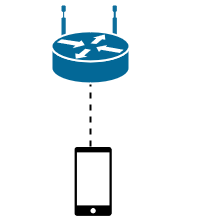
\includegraphics{exper1}
\end{figure}
\begin{itemize}
	\item Router TP-Link TD-W8970
	\begin{center}
		\begin{minipage}{\linewidth}
			Wersja bez przeszkody:\\\\
			\begin{tabular}{|c|c|c|}
				\hline 
				Pomiar & Siła sygnału (w dBm) & Obliczona odległość (w metrach) \\ 
				\hline 
				1 & -41 & 1,16 \\ 
				\hline 
				2 & -40 & 1,04 \\ 
				\hline 
				3 & -37 & 0.73 \\ 
				\hline 
				4 & -42 & 1.30 \\ 
				\hline 
				5 & -37 & 0,73 \\ 
				\hline 
			\end{tabular} 
		\end{minipage} 
	\end{center}
	\begin{center}
		\begin{minipage}{\linewidth}
			Wersja z przeszkodą:\\\\
			\begin{tabular}{|c|c|c|}
				\hline 
				Pomiar & Siła sygnału (w dBm) & Obliczona odległość (w metrach) \\ 
				\hline 
				1 & -38 & 0,82 \\ 
				\hline 
				2 & -39 & 0,92 \\ 
				\hline 
				3 & -42 & 1,30 \\ 
				\hline 
				4 & -46 & 2,07 \\ 
				\hline 
				7 & -43 & 1,46 \\ 
				\hline 
			\end{tabular}				
		\end{minipage} 
	\end{center}
	\item Router TP-Link TL-WA701ND
	\begin{center}
		\begin{minipage}{\linewidth}
			Wersja bez przeszkody:\\\\
			\begin{tabular}{|c|c|c|}
				\hline 
				Pomiar & Siła sygnału (w dBm) & Obliczona odległość (w metrach) \\ 
				\hline 
				1 & -44 & 0,98 \\ 
				\hline 
				2 & -44 & 0,98 \\ 
				\hline 
				3 & -45 & 1,10 \\ 
				\hline 
				4 & -47 & 1,38 \\ 
				\hline 
				5 & -45 & 1,10 \\ 
				\hline 
			\end{tabular} 
		\end{minipage} 
	\end{center}
	\begin{center}
		\begin{minipage}{\linewidth}
			Wersja z przeszkodą:\\\\
			\begin{tabular}{|c|c|c|}
				\hline 
				Pomiar & Siła sygnału (w dBm) & Obliczona odległość (w metrach) \\ 
				\hline 
				1 & -49 & 1,74 \\ 
				\hline 
				2 & -47 & 1,38 \\ 
				\hline 
				3 & -46 & 1,23 \\ 
				\hline 
				4 & -47 & 1,38 \\ 
				\hline 
				5 & -47 & 1,38 \\ 
				\hline 
			\end{tabular}//
		\end{minipage} 
	\end{center}
	\item Samsung Grand 2
	\begin{center}
		\begin{minipage}{\linewidth}
			Wersja bez przeszkody:\\\\
			\begin{tabular}{|c|c|c|}
				\hline 
				Pomiar & Siła sygnału (w dBm) & Obliczona odległość (w metrach) \\ 
				\hline 
				1 & -51 & 1,38 \\ 
				\hline 
				2 & -50 & 1,23 \\ 
				\hline 
				3 & -49 & 1,10 \\ 
				\hline 
				4 & -48 & 0,98 \\ 
				\hline 
				5 & -53 & 1,74 \\ 
				\hline 
			\end{tabular} 
		\end{minipage} 
	\end{center}
	\begin{center}
		\begin{minipage}{\linewidth}
			Wersja z przeszkodą:\\\\
			\begin{tabular}{|c|c|c|}
				\hline 
				Pomiar & Siła sygnału (w dBm) & Obliczona odległość (w metrach) \\ 
				\hline 
				1 & -50 & 1,23 \\ 
				\hline 
				2 & -54 & 1,95 \\ 
				\hline 
				3 & -53 & 1,74 \\ 
				\hline 
				4 & -55 & 2,19 \\ 
				\hline 
				5 & -55 & 2,19 \\ 
				\hline 
			\end{tabular}//
		\end{minipage} 
	\end{center}
\end{itemize}

\subsection{Pomiary zakłóceń}
Eksperyment polegał na rozmieszczeniu trasmiterów na wierzchołkach trójkąta, w środku którego znajdował się odbiornik. Wszystkie urządzenia znajdowały się na tej samej wysokości. Mierzone były zmiany siły sygnału i obliczonej odległości w zależności od kąta położenia odbiornika w stosunku do trasmitera oraz ilości nakładających się na siebie sygnałów. Na początku, włączony był tylko transmiter o indeksie A. Odbiornik znajdował się w stosunku do transmitera pod kątem około 50 stopni. Następnie włączony został transmiter B. Na końcu do modelu został dodany trasmiter C.\\

\begin{figure}				
	\centering
	\caption{Model systemu do pomiaru zakłóceń}
	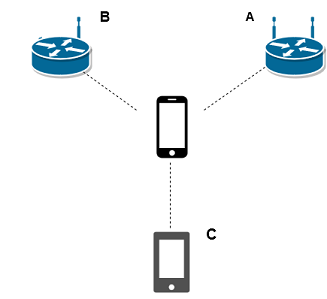
\includegraphics{inz2}
\end{figure}
Informacje o urządzeniach:
\begin{itemize}
	\item Transmiter A - TP-Link TD-W8970, współrzędne (1.80, 0)
	\item Transmiter B - TP-Link TL-WA701ND, współrzędne (0, 0)
	\item Transmiter C - Samsung Grand 2, współrzędne (1.07, 1.8)
	\item Odbiornik - współrzędne (1.2, 0.45)
\end{itemize}
\begin{center}
	\begin{minipage}{\linewidth}
		Pomiar bez zakłóceń dla odległości 80cm przy kącie 50\textdegree :\\\\
		\begin{tabular}{|c|c|c|}
			\hline 
			Pomiar & Siła sygnału (w dBm) & Obliczona odległość (w metrach) \\ 
			\hline 
			1 & -41 & 1,16 \\ 
			\hline 
			2 & -43 & 1,46 \\ 
			\hline 
			3 & -41 & 1,16 \\ 
			\hline 
			4 & -42 & 1,30 \\ 
			\hline 
			5 & -43 & 1,46 \\ 
			\hline 
		\end{tabular}
	\end{minipage} 
\end{center}
\begin{center}
	\begin{minipage}{\linewidth}
		Pomiar z zakłóceniami z transmitera B dla odległości 80cm przy kącie 50\textdegree :\\\\
		\begin{tabular}{|c|c|c|}
			\hline 
			Pomiar & Siła sygnału (w dBm) & Obliczona odległość (w metrach) \\ 
			\hline 
			1 & -44 & 1,64 \\ 
			\hline 
			2 & -47 & 2,31 \\ 
			\hline 
			3 & -45 & 1,84 \\ 
			\hline 
			4 & -48 & 2,60 \\ 
			\hline 
			5 & -47 & 2,31 \\ 
			\hline 
		\end{tabular}
	\end{minipage} 
\end{center}
\begin{center}
	\begin{minipage}{\linewidth}
		Pomiar z zakłóceniami z obu transmiterów dla odległości 80cm przy kącie 50\textdegree :\\\\
		\begin{tabular}{|c|c|c|}
			\hline 
			Pomiar & Siła sygnału (w dBm) & Obliczona odległość (w metrach) \\ 
			\hline 
			1 & -48 & 2,60 \\ 
			\hline 
			2 & -47 & 2,31 \\ 
			\hline 
			3 & -44 & 1,64 \\ 
			\hline 
			4 & -48 & 2,60 \\ 
			\hline 
			5 & -46 & 2,06 \\ 
			\hline 
		\end{tabular}
	\end{minipage} 
\end{center}